% !TEX root = ./Basilisk-houghCircles-20190213.tex

\section{Test Description and Success Criteria}
In order to test the proper function of this module, three test images are provided.
The algorithm needs to find the limbs and match the expected results.

\section{Test Parameters}

For each image, four tests are run:

\begin{table}[htbp]
	\caption{Error tolerance for each test.}
	\label{tab:errortol}
	\centering \fontsize{10}{10}\selectfont
	\begin{tabular}{ c | c  } % Column formatting, 
		\hline\hline
		\textbf{Test}   & \textbf{Absolute Error}  \\  \hline
		Validity Flag           & 1E-5	 [-]  \\ 
		Covariance Values     & 1E-5	[px$^2$]   \\ 
		Number of Limb Points     & 1E-5	[-]   \\ 
		First Limb Point Values     & 1 (Relative Error)	   \\ 
		\hline\hline
	\end{tabular}
\end{table}


\section{Test Results}
The following table shows the results of the unit test described above.

\begin{table}[H]
	\caption{Test results}
	\label{tab:results}
	\centering \fontsize{10}{10}\selectfont
	\begin{tabular}{c | c  } % Column formatting, 
		\hline\hline
		\textbf{Check} 						  		&\textbf{Pass/Fail} \\ 
		\hline
	   MarsBright   			& PASS \\ 
	   MarsDark 			& PASS \\ 
	   Moon   			        & PASS  \\
	   \hline\hline
	\end{tabular}
\end{table}

The test does not generate the result image unless called explicitly from python in order to not add images to the repository.

The Figures draw in red the exact pixel points that are detected at the limb. 

\begin{figure}[h!]
\centering
  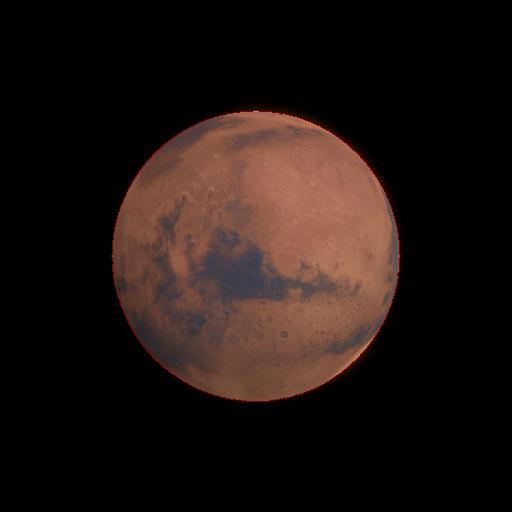
\includegraphics[width = 0.5\linewidth]{../_UnitTest/result_MarsBright.jpg}
  \caption{Mars Circles}
  \label{fig:mars}
\end{figure}

\begin{figure}[h!]
\centering
  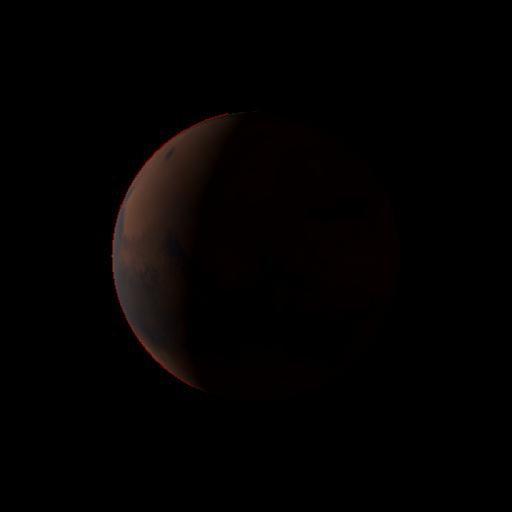
\includegraphics[width = 0.5\linewidth]{../_UnitTest/result_MarsDark.jpg}
  \caption{Mars Circles}
  \label{fig:mars}
\end{figure}

\begin{figure}[h!]
\centering
  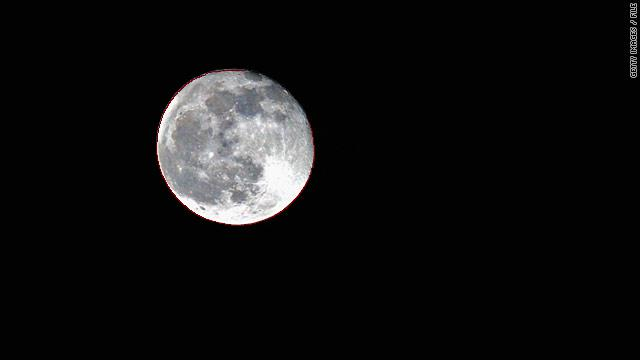
\includegraphics[width = 0.5\linewidth]{../_UnitTest/result_moons.jpg}
  \caption{Moon crescents circles}
  \label{fig:moons}
\end{figure}

